%***********************************************%
%												%
% EECS 470 - Project 1							%
%<------------------> 							%
% Last Modified by:								%
%	William Cunningham on 2014-8-28				%
%												%
%***********************************************%

%***********************************************%
% Preamble										%
%***********************************************%

\documentclass{article}

\usepackage[dvipsnames]{xcolor}

\usepackage{
	tikz,
	colortbl,
	graphicx,
	amsmath,
	amssymb,
	mathrsfs,
	float,
	siunitx,
	fancyhdr,
	url,
	minted,
	cleveref
}


\usepackage
	[left=1in,top=1in,right=1in,bottom=1in]
	{geometry}

\pagestyle{fancy}

%--- Header ---%

\newcommand{\courseNumber}{EECS 470}
\newcommand{\courseTitle}{Computer Architecture}
\newcommand{\university}{University of Michigan, Ann Arbor}
\newcommand{\labdate}{January 21$^{\text{st}}$, 2021}


\lhead{
	\small{
		\university
	}
}
\rhead{
	\small{
		\emph{Date: \labdate} \hspace*{-1em}
		% Why is the above \hspace necessary?
	}
}

\newcommand{\shortbar}{
	\vspace*{-12pt}
	\begin{center}
		\rule{5ex}{0.1pt}
	\end{center}
}
\newcommand{\project}[1]{
	\begin{center}
		\LARGE{
			\vspace*{-12pt}
			EECS 470 Project \##1
			\shortbar
		}
	\end{center}
}


%***********************************************%
%                                               %
% TikZ Definitions                              %
%                                               %
%***********************************************%

\usetikzlibrary{shapes,arrows,automata,shadows}
\pgfdeclarelayer{background}
\pgfdeclarelayer{foreground}
\pgfsetlayers{background,main,foreground}

% Block Diagram Styles
\tikzstyle{block} = [draw, fill=RoyalBlue!50, rectangle,
        minimum height=2cm, minimum width=2cm, rounded corners]
\tikzstyle{sum} = [draw, fill=blue!20, circle, node distance=2cm]
\tikzstyle{input} = [coordinate]
\tikzstyle{output} = [coordinate]
\tikzstyle{branch} = [coordinate]
\tikzstyle{pinstyle} = [pin edge={to-, thin, black}]

% Signal Flow Graph Styles
\tikzstyle{signal} = [draw, fill=RoyalBlue!50, circle,
	minimum height=3em]
\tikzstyle{state} = [draw, fill=RoyalBlue!50, circle,
	minimum height=3em]

%***********************************************%
%                                               %
% Document										%
%                                               %
%***********************************************%

\begin{document}
\vspace*{-20pt}
\project{1}

\begin{itemize}
	\item This is an individual assignment. You may discuss the specification
		and help one another with the (System) Verilog language. Your solution,
		particularly the designs you submit, must be your own.
	\item Due at 11:59pm ET on 30$^{\text{th}}$ January, 2021. \emph{Late submissions are 
		not accepted.}
\end{itemize}
\hrulefill

\section{Introduction}
In this project, you will be designing a number of different priority selectors.
A priority selector, or priority arbiter, has $n$ pairs of request and grant
lines. As the names imply, the selector chooses one of the asserted request
lines and asserts its corresponding grant line. In the most general case, the
selector can assert $k$ grant lines, where $k \le n$, though for this project,
$k=1$. 

Priority selectors are heavily used in computer architecture, where we often
have limited resources that need to be assigned optimally for best performance.
The modules you write for this assignment will both remind you about the
concepts of digital design you first learned in EECS 270 and begin to prepare
you for the final project, where they can be reused. 

\section{Assignment}
In this assignment you will be asked to design and test the following devices:
\begin{itemize}
	\item A 4-bit fixed priority selector
		\begin{itemize}
			\item Using \texttt{assign} statements for the combinational logic.
			\item Using \texttt{always} blocks for the combinational logic.
		\end{itemize}
	\item A 4-bit and an 8-bit fixed priority selector using a hierarchy of
		2-bit selectors.
	\item A 4-bit rotating priority selector using a hierarchy of 2-bit
		selectors.
\end{itemize}

\subsection{Before you start}
Log into a CAEN computer, booted into Redhat Enterprise Linux. Open a terminal,
now run the following commands after downloading project1.tar.gz to your current directory:

% mkdir classes/eecs470/projects
% cd classes/eecs470/projects
% wget eecs.umich.edu/courses/eecs470/projects/project1.tar.gz
\begin{figure}[H]
	\begin{minted}[frame=lines]{bash}
tar -xvf project1.tar.gz
cd project1
	\end{minted}
	\vspace*{-12pt}
	\caption{Project setup guide, from the command line}
\end{figure}

These commands create a directory for 470, create a directory for projects and
then move into that directory. Then, the project 1 source is pulled from the
course website and unpacked. 

\subsection{4-bit Fixed Priority Selector}
For this section, you will design two different 4-bit fixed priority selectors.
Both are to be declared as:

\begin{minted}[frame=lines]{verilog}
module ps4(
    input        [3:0] req,
    input              en,
    output logic [3:0] gnt
);
\end{minted}

The signal \texttt{req[3]} is the highest priority request, and priority goes
down to \texttt{req[0]}, which is the lowest priority request. In all cases no
more than one of the grant lines should be asserted at any given time. If
\texttt{en} is low, then no grant lines should be asserted. For example, if
\texttt{en=1} and \texttt{req=4'b1111}, then \texttt{gnt=4'b1000}.

The design for this section should be put into a file named \texttt{P1a.v}.
Using \texttt{assign} statements (and no \texttt{always} blocks) implement a
4-bit priority selector. You may want to use a K-map to find the logic equations
needed for the grant lines, or you might be able to solve it ad hoc. 

The \texttt{Makefile} provided with this project is already set to use this file
along with a provided testbench, which can be found in the file \texttt{test.v}.
Once you think you have the code correct, simply run the command \texttt{make}
in the directory. Odds are very good that this won't work the first time you try
it, and you'll have to figure out the errors. Compile errors will point you to a
line number in your design, with some kind of hint as to what is wrong. If
things compile it is still possible, perhaps even likely, that the testbench
will find an error. If that happens, you are strongly encouraged to look at the
testbench to try to understand what it is doing. 

Once you have completed the above task, you need to do it again, but this time
put the design in a file named \texttt{P1b.v}. This time you are to use
\texttt{if/else} statements inside an \texttt{always} block. Make the necessary
changes so that the \texttt{Makefile} builds the new file instead of the old
one. 

\subsection{Hierarchical Priority Selectors}

Consider the Verilog you wrote in \texttt{P1a.v} and \texttt{P1b.v}. If you were
going to make a 128-bit priority selector, your design would be quite long and
unreadable. One way to avoid this problem is to build your module in a way that
it can be combined with itself to make a larger version. For example, it is
fairly easy to use three 2-bit \texttt{and} gates to create a single 4-bit
\texttt{and} gate. Think through how you would go about building this.
\Cref{fig:and} shows how this is done in the case of the \texttt{and}. How would
you go about doing this with priority selectors? It's not easy\dots

\begin{figure}[H]
	\centering
	\inputminted[frame=lines,obeytabs,tabsize=4]{verilog}{./and.v}
	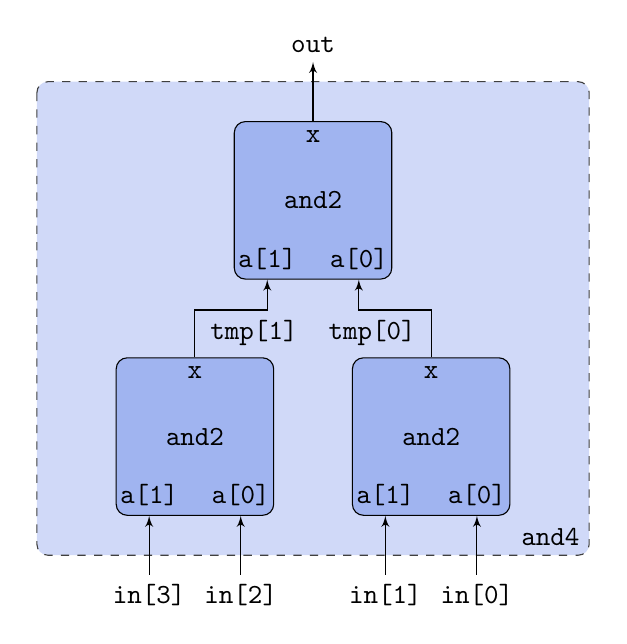
\begin{tikzpicture}[auto, node distance=1.5cm,>=latex',every text node
		part/.style={align=center}]
		\def\blockdist{2em}
		\def\edgedist{2em}

		\begin{pgfonlayer}{foreground}
			\node[block] (top) {\texttt{and2}};
			\node[branch,below of=top,node distance=3cm] (mid) {};
			\node[block,right of=mid] (right) {\texttt{and2}};
			\node[block,left of=mid] (left) {\texttt{and2}};

			\draw[->] (right.north) node[anchor=north] {\texttt{x}} |- +(-0.75cm,0.6cm)
			node[anchor=north] {\texttt{tmp[0]}} -| (top.300) 
			node[anchor=south] {\texttt{a[0]}}; 
			\draw[->] (left.north) node[anchor=north] {\texttt{x}} |- +(+0.75cm,0.6cm) 
			node[anchor=north] {\texttt{tmp[1]}} -| (top.240)
			node[anchor=south] {\texttt{a[1]}}; 
			\draw[<-] (left.240) node[anchor=south] {\texttt{a[1]}} -- +(0cm,-0.75cm)
			node[anchor=north] {\texttt{in[3]}};
			\draw[<-] (left.300) node[anchor=south] {\texttt{a[0]}} -- +(0cm,-0.75cm)
			node[anchor=north] {\texttt{in[2]}};
			\draw[<-] (right.240) node[anchor=south] {\texttt{a[1]}} -- +(0cm,-0.75cm)
			node[anchor=north] {\texttt{in[1]}};
			\draw[<-] (right.300) node[anchor=south] {\texttt{a[0]}} -- +(0cm,-0.75cm)
			node[anchor=north] {\texttt{in[0]}};
			\draw[->] (top.north) node[anchor=north] {\texttt{x}} -- +(0cm,0.75cm) 
			node[anchor=south] {\texttt{out}};
		\end{pgfonlayer}
		\begin{pgfonlayer}{background}
			\path (top.north -| left.west)+(-1,0.5) node (a) {};
			\path (right.east |- right.south)+(1,-0.5) node (b) {};
			\path[fill=RoyalBlue!25, rounded corners, draw=black!75, dashed] (a) rectangle (b);
		\end{pgfonlayer}
		\begin{pgfonlayer}{foreground}
			\draw[] (b) node[anchor=south east] () {\texttt{and4}};
		\end{pgfonlayer}
	\end{tikzpicture}
	\caption{Hierarchical Module Example: a 4-bit \texttt{and} built with three
	2-bit \texttt{and} modules.}
	\label{fig:and}
\end{figure}

Let's consider a 2-bit priority selector as a building block. In order to make
a 4-bit device, you'd need three of 2-bit selectors in a tree structure, similar
the \texttt{and}'s above. The right might get the two lowest priority request
and grant lines, while the left got the two highest priority request and grant
lines. Then the left and right would ask the top to choose which of them got the
grant. In our previous 4-bit module we had a way to be told if we \emph{could}
grant to anyone, the enable line (\texttt{en}).  But we didn't have a way of
saying ``Hey, I have a request that would like a grant.'' We will need to add
that functionality, and you should call it \texttt{req\_up} for ``requesting
something from the device above me.'' This signal should be asserted if either
request is asserted no matter the value of the enable. 

You will need two modules, one is the 2-bit priority selector and the other is
the 4-bit. These modules should be declared as follows:

\begin{figure}[H]
\begin{minted}[frame=lines]{verilog}
module ps2(
	input        [1:0] req,
	input              en,
	output logic [1:0] gnt,
	output logic       req_up
);

module ps4(
	input        [3:0] req,
	input              en,
	output logic [3:0] gnt,
	output logic       req_up
);
\end{minted}
\end{figure}

To build the 2-bit selector, use either \texttt{P1a.v} or
\texttt{P1b.v} as a template, and don't forget to include the \texttt{req\_up}
signal. Then you need to build the 4-bit device. Use \cref{fig:and} as an
example of the concept of the tree structure, and in particular, be sure you 
understand the Verilog before you proceed.

Your design for this section should be written into a file named \texttt{P1c.v}.
In addition, you will need to modify the testbench to use this new module and
its additional output. Make the needed changes to the Makefile to use this new
design. Once you have this version working, build a \texttt{ps8} module using
\texttt{ps4} and \texttt{ps2} modules, and save it in the same file. The module
declarations should follow from \texttt{ps4}, above. For full credit, your design
should not contain any additional ``glue`` logic. It should only contain the
minimum number of ps modules and wires connecting them. To test this new
module, write a new testbench and save it as \texttt{testC.v}. You will need to
turn it in.

\subsection{Hierarchical Rotating Priority Selectors}
It is often the case that you would like to evenly service all devices connected
to some common resource, instead of prioritizing one over the another. This
avoids \emph{livelock} where a lower priority device is never selected because
something with higher priority is constantly requesting. One way to build such a
selector is to change priority every clock tick. To do this, we clearly need to
introduce some sequential logic.

\begin{figure}[h]
	\centering
	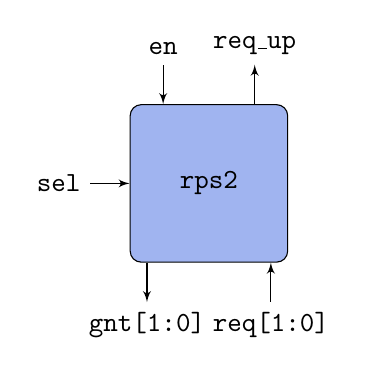
\begin{tikzpicture}[auto, node distance=1.5cm,>=latex', every text node
		part/.style={align=center}]
		\def\blockdist{2em}
		\def\edgedist{2em}
		\begin{pgfonlayer}{foreground}
			\node[block] (rps2) {\texttt{rps2}};

			\draw[<-] (rps2.120)  --+(0cm,0.5cm)  node[anchor=south] {\texttt{en}}      ;
			\draw[->] (rps2.60)   --+(0cm,0.5cm)  node[anchor=south] {\texttt{req\_up}} ;
			\draw[<-] (rps2.west) --+(-0.5cm,0cm) node[anchor=east]  {\texttt{sel}}     ;
			\draw[->] (rps2.232)  --+(0cm,-0.5cm) node[anchor=north] {\texttt{gnt[1:0]}};
			\draw[<-] (rps2.308)  --+(0cm,-0.5cm) node[anchor=north] {\texttt{req[1:0]}};
		\end{pgfonlayer}
		%\begin{pgfonlayer}{background}
			%\path (rps2.north -| rps2.west)+(-1,0.5) node (a) {};
			%\path (rps2.east |- rps2.south)+(1,-0.5) node (b) {};
			%\path[fill=RoyalBlue!25, rounded corners, draw=black!75, dashed] (a) rectangle (b);
		%\end{pgfonlayer}
	\end{tikzpicture}
	\caption{2-bit rotating priority selector (\texttt{rps2})}
\end{figure}

In this case, \texttt{sel} chooses which bit of the \texttt{req} bus will have 
the higher priority. For this assignment, if \texttt{sel=1}, then 
\texttt{req[1]} has the higher priority.

\begin{figure}[h]
	\centering
	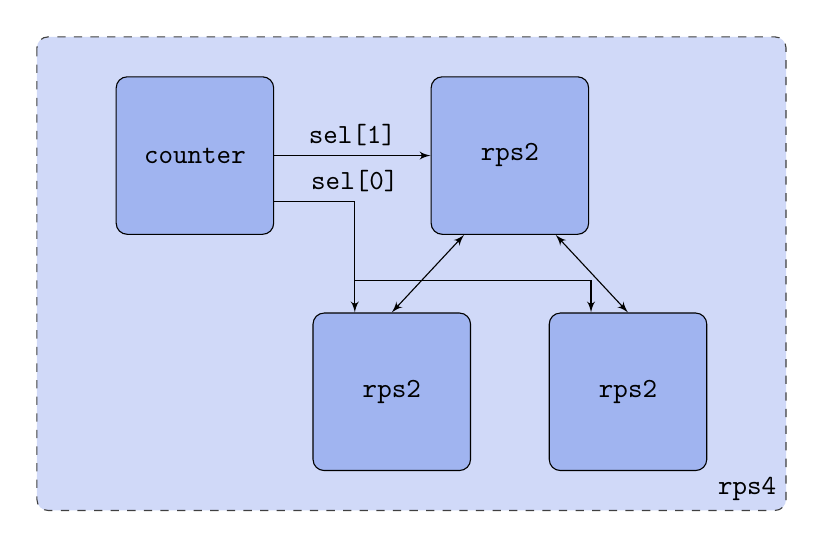
\begin{tikzpicture}[auto, node distance=1.5cm,>=latex', every text node
		part/.style={align=center}]
		\def\blockdist{2em}
		\def\edgedist{2em}

		\begin{pgfonlayer}{foreground}
			\node[block] (top) {\texttt{rps2}};
			\node[branch,below of=top,node distance=3cm] (mid) {};
			\node[block,right of=mid] (right) {\texttt{rps2}};
			\node[block,left of=mid] (left) {\texttt{rps2}};
			\node[block,left of=top,node distance=4cm] (cnt) {\texttt{counter}};
			
			%\draw[<->] (right.north) node[anchor=north] {} |- +(-0.75cm,0.6cm)
			%node[anchor=north] {} -| (top.300) 
			%node[anchor=south] {}; 
			%\draw[<->] (left.north) node[anchor=north] {} |- +(+0.75cm,0.6cm) 
			%node[anchor=north] {} -| (top.240)
			%node[anchor=south] {}; 
			\draw[<->] (top.300) -- (right.north);
			\draw[<->] (top.240) -- (left.north);
			\draw[->] (cnt.east) -- node[pos=0.5,anchor=south] {\texttt{sel[1]}}
			(top.west);
			\draw[->] (cnt.330) -| node[pos=0.5,anchor=south] (anch) {\texttt{sel[0]}}
			(left.115);
			%\draw[->] (cnt.330) -| +(0.9cm,-0.75cm) -| (right.120);
			\draw[->] (anch.south) |- +(0cm,-1cm) -| (right.115);
			
		\end{pgfonlayer}

		\begin{pgfonlayer}{background}
			\path (cnt.north -| cnt.west)+(-1,0.5) node (a) {};
			\path (right.east |- right.south)+(1,-0.5) node (b) {};
			\path[fill=RoyalBlue!25, rounded corners, draw=black!75, dashed] (a) rectangle (b);
		\end{pgfonlayer}
		\begin{pgfonlayer}{foreground}
			\draw[] (b) node[anchor=south east] () {\texttt{rps4}};
		\end{pgfonlayer}
	\end{tikzpicture}
	\caption{Submodules of the 4-bit rotating priority selector}
	\label{fig:rps4}
\end{figure}

\Cref{fig:rps4} shows how the \texttt{sel} bus should be used in the 4-bit
selector. Each level of the tree uses the same bit of the bus. The design for
the \texttt{rps4} and \texttt{rps2} modules should go in a file called
\texttt{P1d.v}. You should use \texttt{P1c.v} as a starting point by adding a
select line to the \texttt{ps2} module and renaming \texttt{ps4} to
\texttt{rps4}. Additionally, \texttt{rps4} will need 1-bit \texttt{clock} and
\texttt{reset} lines, and a 2-bit \texttt{count} output. The module declaration
is as follows:

\begin{figure}[H]
\begin{minted}[frame=lines]{verilog}
module rps4(
	input              clock,
	input              reset,
	input        [3:0] req,
	input              en,
	output logic [3:0] gnt,
	output logic [1:0] count
);
\end{minted}
\end{figure}

A testbench, named \texttt{testD.v}, has been provided with this project. Be
sure you've followed the directions above about which bit of the \texttt{sel}
bus to route where and exactly how this bus works. In all cases, the testbench
needs to be passed\dots

\subsection{Additional Thoughts}
If you get extra time, here are some things that you \emph{should} look into. No
points will be given for any of this.
\begin{itemize}
	\item What is the \texttt{correct} signal doing in the testbench?
	\item In \texttt{testD.v}, there is a \#6. What happens if you replace that with a \#10? Why?
	\item Using a counter, you could do exhaustive testing (test every possible
		case) for the fixed priority devices. You could do it for the rotating
		ones too, but it would be harder. In general, when is exhaustive testing
		\emph{not} a good idea?
	\item There is a \texttt{\$random} function provided in Verilog for testing,
		which can be used to generate random test vectors. Read about it online
		and try to understand how it works. Why would you want to use this
		function?
\end{itemize}
\section{Submission}
After you are confident in your solution, make sure you have the following files
in your directory
\begin{enumerate}
	\item \texttt{P1a.v}
	\item \texttt{P1b.v}
	\item \texttt{P1c.v}
	\item \texttt{P1d.v}
	\item \texttt{testC.v}
\end{enumerate}
Now, go up one directory (\texttt{cd ..}) and run:

\texttt{/afs/umich.edu/user/j/b/jbbeau/Public/470submit -p1 <directory>}

\noindent
Note that the script takes a directory name as an argument, not an absolute
path, so \textbf{you must run it from one level above your project 1 directory}. 

At this point, you should see something similar to: 
\inputminted[frame=lines,obeytabs,tabsize=4]{bash}{submission.txt}
\noindent
If there is a problem, it will be printed to the screen. Shortly after
submission you should receive an email telling you if your submission passed the
basic tests. This is not an autograder, so it's simply telling you that your
design built successfully on the grading machine and that the module
declarations looked approximately correct. If your submission didn't pass, copy
the error message into an email to the course staff, and we will attempt to
help.

Remember that for all projects in this class, you design must have proper simulation output after synthesis as well as before.
\end{document}

